%%
%% Automatically generated file from DocOnce source
%% (https://github.com/hplgit/doconce/)
%%
%%


%-------------------- begin preamble ----------------------

\documentclass[%
oneside,                 % oneside: electronic viewing, twoside: printing
final,                   % draft: marks overfull hboxes, figures with paths
10pt]{article}

\listfiles               %  print all files needed to compile this document

\usepackage{relsize,makeidx,color,setspace,amsmath,amsfonts,amssymb}
\usepackage[table]{xcolor}
\usepackage{bm,ltablex,microtype}

\usepackage[pdftex]{graphicx}

\usepackage[T1]{fontenc}
%\usepackage[latin1]{inputenc}
\usepackage{ucs}
\usepackage[utf8x]{inputenc}

\usepackage{lmodern}         % Latin Modern fonts derived from Computer Modern

% Hyperlinks in PDF:
\definecolor{linkcolor}{rgb}{0,0,0.4}
\usepackage{hyperref}
\hypersetup{
    breaklinks=true,
    colorlinks=true,
    linkcolor=linkcolor,
    urlcolor=linkcolor,
    citecolor=black,
    filecolor=black,
    %filecolor=blue,
    pdfmenubar=true,
    pdftoolbar=true,
    bookmarksdepth=3   % Uncomment (and tweak) for PDF bookmarks with more levels than the TOC
    }
%\hyperbaseurl{}   % hyperlinks are relative to this root

\setcounter{tocdepth}{2}  % levels in table of contents

% Tricks for having figures close to where they are defined:
% 1. define less restrictive rules for where to put figures
\setcounter{topnumber}{2}
\setcounter{bottomnumber}{2}
\setcounter{totalnumber}{4}
\renewcommand{\topfraction}{0.95}
\renewcommand{\bottomfraction}{0.95}
\renewcommand{\textfraction}{0}
\renewcommand{\floatpagefraction}{0.75}
% floatpagefraction must always be less than topfraction!
% 2. ensure all figures are flushed before next section
\usepackage[section]{placeins}
% 3. enable begin{figure}[H] (often leads to ugly pagebreaks)
%\usepackage{float}\restylefloat{figure}

% prevent orhpans and widows
\clubpenalty = 10000
\widowpenalty = 10000

% --- end of standard preamble for documents ---


% insert custom LaTeX commands...

\raggedbottom
\makeindex
\usepackage[totoc]{idxlayout}   % for index in the toc
\usepackage[nottoc]{tocbibind}  % for references/bibliography in the toc

%-------------------- end preamble ----------------------

\begin{document}

% matching end for #ifdef PREAMBLE

\newcommand{\exercisesection}[1]{\subsection*{#1}}


% ------------------- main content ----------------------



% ----------------- title -------------------------

\thispagestyle{empty}

\begin{center}
{\LARGE\bf
\begin{spacing}{1.25}
Project 5, deadline  December 10, 2017
\end{spacing}
}
\end{center}

% ----------------- author(s) -------------------------

\begin{center}
{\bf Partial Differential equations${}^{}$} \\ [0mm]
\end{center}

\begin{center}
% List of all institutions:
\end{center}
    
% ----------------- end author(s) -------------------------

% --- begin date ---
\begin{center}
Fall semester 2017
\end{center}
% --- end date ---

\vspace{1cm}


\subsection*{Theoretical background and description of the system}

This project is more numerically directed, with tests
of algorithms for solving partial differential equations using finite difference schemes. 
Chapter 10 of the lecture notes provides the necessary theoretical background.

\textbf{For this project you can collaborate with fellow students and you can  hand in a common report.}
This project (together with projects 3 and 4) counts 1/3 of the final mark.

The project has a strong mathematical axis. However, for those interested, it should be straightforward to replace the dimensionless analysis in  parts 5a-5f) with specific boundary and initial conditions. This is done in part 5g), with a focus on the heat equation and geophysical processes. That part is optional, but gives an additional 30 points to a score of 100.

The physical problem can be that of the temperature gradient in a rod of length $L=1$ or that of channel flow
between two flat and infinite plates at $x=0$ and $x=1$, where the fluid is initially at rest
and the plate $x=1$ is given a sudden initial movement.  We are looking at a one-dimensional
problem

\begin{equation*}
 \frac{\partial^2 u(x,t)}{\partial x^2} =\frac{\partial u(x,t)}{\partial t}, t> 0, x\in [0,L]
\end{equation*}
or

\begin{equation*}
u_{xx} = u_t,
\end{equation*}
with initial conditions, i.e., the conditions at $t=0$,

\begin{equation*}
u(x,0)= 0 \hspace{0.5cm} 0 < x < L
\end{equation*}
with $L=1$ the length of the $x$-region of interest. The 
boundary conditions are

\begin{equation*}
u(0,t)= 0 \hspace{0.5cm} t \ge 0,
\end{equation*}
and

\begin{equation*}
u(L,t)= 1 \hspace{0.5cm} t \ge 0.
\end{equation*}
The function $u(x,t)$  can be the temperature gradient of a  rod or represent the fluid velocity 
in a direction parallel to the plates, that is normal to the $x$-axis. In the latter case, 
for small $t$, only the part of the fluid
close to the moving plate is set in significant  motion, resulting in a thin boundary layer at $x=1$. 
As time increases, the velocity approaches a linear variation with $x$. In this case, which can be derived
from the incompressible Navier-Stokes, the above equations constitute a model for  
studying friction between moving surfaces separated by a thin fluid film.

In this project we want to study the numerical stability of three methods for partial differential equations
(PDEs). 
These methods we will discuss are
the explicit forward Euler algorithm with discretized versions of time given by a forward formula and a centered difference in space resulting in   
\begin{equation*} 
u_t\approx \frac{u(x,t+\Delta t)-u(x,t)}{\Delta t}=\frac{u(x_i,t_j+\Delta t)-u(x_i,t_j)}{\Delta t}
\end{equation*}
and

\begin{equation*}
u_{xx}\approx \frac{u(x+\Delta x,t)-2u(x,t)+u(x-\Delta x,t)}{\Delta x^2},
\end{equation*}
or

\begin{equation*}
u_{xx}\approx \frac{u(x_i+\Delta x,t_j)-2u(x_i,t_j)+u(x_i-\Delta x,t_j)}{\Delta x^2}.
\end{equation*}
We will also discuss the implicit Backward Euler with   
\begin{equation*} 
u_t\approx \frac{u(x,t)-u(x,t-\Delta t)}{\Delta t}=\frac{u(x_i,t_j)-u(x_i,t_j-\Delta t)}{\Delta t}
\end{equation*}
and

\begin{equation*}
u_{xx}\approx \frac{u(x+\Delta x,t)-2u(x,t)+u(x-\Delta x,t)}{\Delta x^2},
\end{equation*}
or

\begin{equation*}
u_{xx}\approx \frac{u(x_i+\Delta x,t_j)-2u(x_i,t_j)+u(x_i-\Delta x,t_j)}{\Delta x^2},
\end{equation*}

Finally we use the implicit Crank-Nicolson scheme with  a time-centered scheme at $(x,t+\Delta t/2)$   
\begin{equation*} 
u_t\approx \frac{u(x,t+\Delta t)-u(x,t)}{\Delta t}=\frac{u(x_i,t_j+\Delta t)-u(x_i,t_j)}{\Delta t}.
\end{equation*}
The corresponding spatial second-order derivative reads

\begin{align*}
u_{xx}\approx &\frac{1}{2}\left(\frac{u(x_i+\Delta x,t_j)-2u(x_i,t_j)+u(x_i-\Delta x,t_j)}{\Delta x^2}\right. +\\
&\left. \frac{u(x_i+\Delta x,t_j+\Delta t)-2u(x_i,t_j+\Delta t)+u(x_i-\Delta x,t_j+\Delta t)}{\Delta x^2}\right).
\end{align*}
Note well that we are using a time-centered scheme wih $t+\Delta t/2$ as center.



\paragraph{Project 5a): Setting up the algorithms.}
Write down the algorithms for these three methods and the equations you need to implement.
For the implicit schemes show that the equations lead to a tridiagonal matrix system for the new values.

\paragraph{Project 5b): Truncation errors and analytic solutions.}
Find the truncation errors of these three schemes and investigate their stability properties.
Find also the analytic solution to the continuous problem. 

\paragraph{Project 5c): Implementation.}
Implement the three algorithms in the same code and perform tests of the solution 
for these three approaches
for $\Delta x=1/10$, $\Delta x=1/100$ using  $\Delta t$ as dictated by the stability limit of the explicit scheme.
Study the solutions at two time points $t_1$ and $t_2$ where $u(x,t_1)$ is smooth but still significantly curved
and $u(x,t_2)$ is almost linear, close to the stationary state.
Remember that forsolving the tridiagonal equations you can use your code from project 1.  
\paragraph{Project 5d):}
Compare the solutions at $t_1$ and $t_2$ with the analytic result for the continuous problem.
Which of the schemes would you classify as the best?

\paragraph{Project 5e): Moving to two dimensions.}
Extend the code you have developed here to two
  dimensions. 
It means that we deal with a $2+1$ dimensional problem. Our differential equation becomes
\[
 \frac{\partial^2 u(x,y,t)}{\partial x^2}+\frac{\partial^2 u(x,y,t)}{\partial y^2} =\frac{\partial u(x,y,t)}{\partial t}, t> 0, x,y\in [0,1],
\]
where we now have made a model with a square lattice for $x$ and $y$. 
How would you extend the boundary conditions from one dimension to two dimensions? And can you
  find a closed form solution here as well?  It is left to you to decide upon what kind of boundary conditions
you deem appropriate.
\paragraph{Project 5f): Solving the two-dimensional equations numerically.}
Here you can choose between an explicit or an implicit scheme. 
For the implicit scheme discussed in chapter 10 of the lecture notes, upi need to use for example an iterative method like Jacobi's.

Outline the algorithm for solving the two-dimensional diffusion equation and 
implement the explicit or the implicit scheme as function of $\Delta x$ (assuming
$\Delta x = \Delta y$) and $\Delta t$. Solve the equations numerically and give a critical discussion of your results. 
Compare your results with the closed-form answer. Discuss the stability
of the solution as function of different values of $\Delta x$  and $\Delta t$. 

You should, if you have time, try to  parallelize the equations using MPI or OpenMP. 


\paragraph{Project 5g) Temperature distribution in the lithosphere (this part is optional and gives an additional score of 30 points).}
The Scientific background is  based on geological evidence at the surface. Geologists have proposed
that there was an active subduction zone on the western coast of
Norway about 1Gy ago. When subducting, the oceanic lithosphere
releases water and other chemical components that go mostly to the
surface but may also be trapped in the mantle above the subducting
slab. This process is called the refertilization of the mantle wedge
(see Figure). These chemical components contain more radioactive
elements than the normal mantle. We can therefore expect that ancient
mantle wedges are enriched in radioactive elements and therefore
warmer than normal mantle. The question is how much warmer they are
and if we can find evidence for this enrichment in geophysical
studies.

\begin{figure}[!ht]  % 
  \centerline{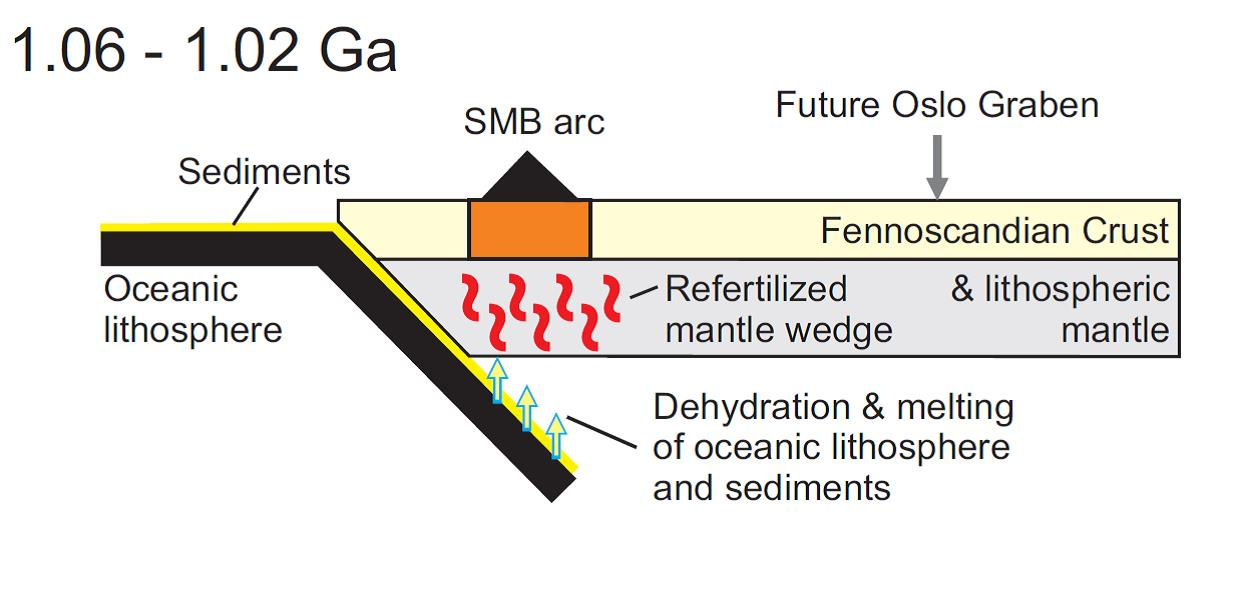
\includegraphics[width=0.6\linewidth]{figslides/slab.jpg}}
  \caption{
  Cartoon of the enrichment of the mantle by a subduction slab.
  }
\end{figure}
%\clearpage % flush figures 


The purpose of this part is to 
calculate the thermal evolution of the lithosphere up to present following the emplacement of radioactive elements in the mantle wedge 1 Gy ago.

The equation to compute is the time evolution of the temperature distribution is the heat equation, which will be used only in 2D here, namely

\begin{equation}
\vec \nabla(k \vec \nabla T) + Q = \rho c_p \frac{\partial T}{\partial t} 
\label{eq:heat2D}
\end{equation}
where $T$ is the temperature, $\rho$ is the density, $k$ is the thermal conductivity, $c_p$ is the specific heat capacity and $Q$ is the heat production.

With the boundary conditions and initial conditions, you should rescale your equations in order to use the results from parts 5a-5f). The paramaters of the model are described here.

\paragraph{Parameters of the model.}
The boundary conditions are $8^{\circ}\,C$ at the surface and $1300^{\circ}C$ at the bottom at a depth of 120 km.

In this study, we assume a constant density for the lithosphere of $3.5 10^3\,Kg/m^3$,
a constant thermal conductivity of $2.5\,W/m/^{\circ}C$
and a constant specific heat capacity of $1000\,J/Kg/^{\circ}C^{-1}$.

The heat production, caused by radioactive decay, cannot be taken as uniform in the whole lithosphere as radioactive elements are much more abundant in the crust than in the mantle.
We need therefore to separate the lithosphere in 3 units: the upper crust from 0 to 20 km depth, the lower crust from 20 to 40 km depth and the mantle from 40 to 120 km depth, where the heat production is set respectively to $1.4\,\mu W/m^3$, $0.35\,\mu W/m^3$ and $0.05\,\mu W/m^3$. 

\paragraph{Temperature distribution before radioactive enrichment.}
Before radioactive enrichment, the temperature is steady-state and depends only on depth. In order to test your results you should
try to obtain analytical results for  the temperature profile as function of depth neglecting the presence of radioactice sources and. Compare thereafter these results with your numerical results.  Include then the radioactive sources and compare eventual analytical results with numerical calculations.

\paragraph{Temperature distribution after radioactive enrichment.}
We assume that the lithosphere above the slab gets enriched in
radioactive elements U, Th and K 1 Gy ago and that this results in an
additional heat production of $0.5\mu W/m^3$ over the whole depth of
the mantle (not the crust) in a 150 km wide area above the
slab. Neglecting all other thermal perturbations that this slab could
produce, and assuming that the heat production will remain constant
over geological time, compute the thermal evolution of the lithosphere
from 1 Gy to present.

The radioactivity will decrease with time. Assuming that the
additional heat is produced at 40\% by U, 40\% by Th and 20\% by K,
which have halflives of 4.47 Gy, 14.0 Gy and 1.25 Gy respectively,
compute the thermal evolution of the lithosphere and compare with the
result obtained above.






\paragraph{References.}
A very good reference is the textbook by \href{{http://www.springer.com/us/book/9783540225515}}{Winther and Tveito on partial differential equations}. It is available online \href{{https://vpn2.uio.no/+CSCO+0h756767633A2F2F797661782E66636576617472652E70627A++/book/10.1007/b138016/page/1}}{from the University library}.


\subsection*{Introduction to numerical projects}

Here follows a brief recipe and recommendation on how to write a report for each
project.

\begin{itemize}
  \item Give a short description of the nature of the problem and the eventual  numerical methods you have used.

  \item Describe the algorithm you have used and/or developed. Here you may find it convenient to use pseudocoding. In many cases you can describe the algorithm in the program itself.

  \item Include the source code of your program. Comment your program properly.

  \item If possible, try to find analytic solutions, or known limits in order to test your program when developing the code.

  \item Include your results either in figure form or in a table. Remember to        label your results. All tables and figures should have relevant captions        and labels on the axes.

  \item Try to evaluate the reliabilty and numerical stability/precision of your results. If possible, include a qualitative and/or quantitative discussion of the numerical stability, eventual loss of precision etc.

  \item Try to give an interpretation of you results in your answers to  the problems.

  \item Critique: if possible include your comments and reflections about the  exercise, whether you felt you learnt something, ideas for improvements and  other thoughts you've made when solving the exercise. We wish to keep this course at the interactive level and your comments can help us improve it.

  \item Try to establish a practice where you log your work at the  computerlab. You may find such a logbook very handy at later stages in your work, especially when you don't properly remember  what a previous test version  of your program did. Here you could also record  the time spent on solving the exercise, various algorithms you may have tested or other topics which you feel worthy of mentioning.
\end{itemize}

\noindent
\subsection*{Format for electronic delivery of report and programs}

The preferred format for the report is a PDF file. You can also use DOC or postscript formats or as an ipython notebook file.  As programming language we prefer that you choose between C/C++, Fortran2008 or Python. The following prescription should be followed when preparing the report:

\begin{itemize}
  \item Use Devilry to hand in your projects, log in  at  \href{{http://devilry.ifi.uio.no}}{\nolinkurl{http://devilry.ifi.uio.no}} with your normal UiO username and password and choose either 'fys3150' or 'fys4150'. There you can load up the files within the deadline.

  \item Upload \textbf{only} the report file!  For the source code file(s) you have developed please provide us with your link to your github domain.  The report file should include all of your discussions and a list of the codes you have developed.  Do not include library files which are available at the course homepage, unless you have made specific changes to them.

  \item In your git repository, please include a folder which contains selected results. These can be in the form of output from your code for a selected set of runs and input parametxers.

  \item In this and all later projects, you should include tests (for example unit tests) of your code(s).

  \item Comments  from us on your projects, approval or not, corrections to be made  etc can be found under your Devilry domain and are only visible to you and the teachers of the course.
\end{itemize}

\noindent
Finally, 
we encourage you to work two and two together. Optimal working groups consist of 
2-3 students. For this specific report you can  hand in a common report.














% ------------------- end of main content ---------------

\end{document}

